\documentclass{lib/skripsi}

\usepackage{blindtext}
%===========================================================
% Definisi Data Peneliti, Judul, Pembimbing dan Penguji
%-----------------------------------------------------------
\typedocument{proposal skripsi}
\titleskripsi{MEDIA PEMBELAJARAN PENGOLAHAN CITRA DIGITAL MENGGUNAKAN VISUALISASI INTERAKTIF BERBASIS WEB}

\fullname{RAHMAT ARDIANSYAH}
\npm{193510147}

\yearsubmit{2023}
\program{Teknik Informatika}
\faculty{Teknik}
\university{Universitas Islam Riau}
\city{Pekanbaru}

%-----------------------------------------------------------
% End Definisi Data Peneliti, Judul, Pembimbing dan Penguji
%===========================================================

\begin{document}
    \coverproposal
    \pagenumbering{roman}

    %===========================================================
    % Kata Pengantar, Daftar isi, daftar gambar, daftar tabel
    %-----------------------------------------------------------
    \frenchspacing
    \addcontentsline{toc}{chapter}{KATA PENGANTAR}
\chapter*{KATA PENGANTAR}

Puji syukur kehadirat Allah SWT yang telah memberikan rahmat dan hidayah-Nya sehingga penulis dapat menyelesaikan proposal tugas akhir yang berjudul ``\textbf{Media Pembelajaran Pengolahan Citra Menggunakan Visualisasi Interaktif Berbasis Web}''. Proposal tugas akhir ini disusun sebagai salah satu langkah awal dalam menyelesaikan program studi Sarjana Teknik Informatika.

Penulis menyadari bahwa pembuatan media pembelajaran ini tidak mudah, karena dibutuhkan pemahaman yang cukup tentang pengolahan citra digital dan teknologi web. Namun, dengan bimbingan dan dukungan dari dosen pembimbing, penulis yakin dapat menyelesaikan tugas akhir ini dengan baik.

Akhir kata, penulis mengucapkan terima kasih kepada semua pihak yang telah membantu dan mendukung penulis dalam menyelesaikan proposal tugas akhir ini.

\vspace{1cm}
\begin{flushright}
    Pekanbaru, 1 Juli 2024\\
    \vspace{2.5cm}
    {RAHMAT ARDIANSYAH}\\
\end{flushright}


    \pagebreak

    \addcontentsline{toc}{chapter}{DAFTAR ISI}
    \tableofcontents
    \pagebreak

    % \addcontentsline{toc}{chapter}{DAFTAR TABEL}
    % \listoftables
    % \pagebreak

    \addcontentsline{toc}{chapter}{DAFTAR GAMBAR}
    \listoffigures
    \pagebreak

    \pagenumbering{arabic}
    %-----------------------------------------------------------
    % End Daftar isi, daftar gambar, daftar tabel
    %===========================================================

    %===========================================================
    % Daftar masukan untuk Bab
    %-----------------------------------------------------------
    \chapter{PENDAHULUAN}

\section{Latar Belakang}
Pengolahan citra digital telah menjadi bidang yang semakin penting dalam era digital ini. Dalam berbagai bidang seperti ilmu komputer, grafika komputer, pengenalan pola, penglihatan komputer, dan banyak aplikasi lainnya, pengolahan citra digital berperan penting dalam analisis, manipulasi, dan interpretasi gambar digital.

Pada saat yang sama, perkembangan teknologi informasi dan komunikasi (TIK) telah membawa dampak signifikan dalam dunia pendidikan. Pemanfaatan media pembelajaran dalam proses pendidikan telah menjadi semakin umum, dan penggunaan media berbasis web menjadi salah satu tren yang semakin populer. Media berbasis web memiliki keunggulan dalam aksesibilitas dan fleksibilitasnya yang tinggi, yang memungkinkan mahasiswa untuk mengakses dan berinteraksi dengan materi pembelajaran secara efektif.

Dalam konteks ini, penelitian ini bertujuan untuk mengembangkan sebuah media pembelajaran pengolahan citra digital yang menggunakan visualisasi interaktif berbasis web. Dengan memanfaatkan potensi media berbasis web, penelitian ini bertujuan untuk menyediakan alat yang interaktif dan dinamis bagi mahasiswa untuk belajar dan mengajarkan konsep pengolahan citra digital secara lebih efektif.

Media pembelajaran yang diusulkan akan memberikan visualisasi yang menarik dan interaktif untuk membantu pemahaman konsep-konsep dasar dalam pengolahan citra digital. Mahasiswa akan dapat berinteraksi dengan gambar dan algoritma pengolahan citra, memanipulasi parameter, dan melihat hasil transformasi citra secara langsung melalui antarmuka berbasis web yang ramah pengguna.

Dengan adanya media pembelajaran ini, diharapkan siswa akan lebih terlibat dan tertarik dalam proses pembelajaran pengolahan citra digital. Selain itu, dosen juga akan mendapatkan alat yang berguna untuk mengajarkan konsep-konsep ini dengan cara yang lebih menarik dan mudah dipahami.

Penelitian ini diharapkan dapat memberikan kontribusi dalam pengembangan media pembelajaran yang inovatif dan interaktif dalam bidang pengolahan citra digital. Dengan meningkatkan kualitas pembelajaran di bidang ini, diharapkan dapat mempersiapkan mahasiswa untuk menghadapi tantangan dan peluang di dunia yang semakin digital.

\section{Identifikasi Masalah}
Berikut adalah beberapa identifikasi masalah yang dapat diambil dari latar belakang di atas:

\begin{enumerate}
  \item Saat ini, masih terbatasnya media pembelajaran berbasis web yang interaktif dalam pengolahan citra digital.
  \item  Kurangnya aksesibilitas dan fleksibilitas. Beberapa media pembelajaran pengolahan citra digital mungkin hanya tersedia dalam bentuk cetak atau terbatas pada platform tertentu.
  \item Pengolahan citra digital melibatkan konsep-konsep yang kompleks dan abstrak.
\end{enumerate}

\section{Rumusan Masalah}
Berdasarkan latar belakang di atas, maka dapat dirumuskan masalah utama dari proposal tugas akhir ini sebagai berikut:

Bagaimana mengembangkan media pembelajaran pengolahan citra digital yang lebih interaktif dan mudah dipahami oleh mahasiswa dengan memanfaatkan teknologi web dan visualisasi interaktif?

Untuk menjawab masalah tersebut, diperlukan beberapa pertanyaan penelitian yang lebih spesifik, yaitu:

\begin{enumerate}
    \item Apa saja konsep-konsep dasar yang harus dipahami oleh mahasiswa dalam pembelajaran pengolahan citra digital?
    \item Bagaimana mengembangkan media pembelajaran pengolahan citra digital yang interaktif dan mudah dipahami dengan memanfaatkan teknologi web dan visualisasi interaktif?
    \item Bagaimana mengukur efektivitas media pembelajaran yang telah dikembangkan?
    \item Bagaimana tingkat kepuasan mahasiswa terhadap penggunaan media pembelajaran yang dikembangkan?
\end{enumerate}

\section{Batasan Masalah}

Dalam penelitian ini, terdapat beberapa batasan masalah yang perlu diperhatikan. Batasan-batasan tersebut adalah:

\begin{enumerate}
    \item Penelitian ini akan difokuskan pada pengolahan citra digital sebagai subjek utama dalam media pembelajaran yang diusulkan. Lingkup pengolahan citra digital meliputi konsep segmentasi seperti operator \textit{Roberts}, operator \textit{Prewitt}, operator \textit{Sobel}, operator \textit{Laplacian} dan operator \textit{Canny}.
    \item Media pembelajaran akan dikembangkan dalam bentuk aplikasi berbasis web sehingga dapat diakses dengan mudah melalui berbagai perangkat.
    \item Aplikasi media pembelajaran yang dikembangkan akan memiliki beberapa fungsi dan fitur, seperti tampilan interaktif, kontrol dan manipulasi citra, dan pemrosesan citra secara \textit{real-time}.
    \item Pengembangan media pembelajaran pengolahan citra digital dengan visualisasi interaktif berbasis web ini akan dilakukan dalam waktu tertentu, sehingga batasan waktu pengembangan akan menjadi salah satu batasan yang harus diperhatikan dalam tugas akhir ini.
\end{enumerate}

\section{Tujuan Penelitian}
Tujuan dari penelitian tugas akhir ini adalah untuk mengembangkan media pembelajaran yang lebih interaktif dan mudah dipahami dengan memanfaatkan teknologi web dan visualisasi interaktif. Selain itu, penelitian ini juga bertujuan untuk meningkatkan kualitas pembelajaran pengolahan citra digital dan mempermudah mahasiswa dalam memahami konsep-konsep yang kompleks dan abstrak. Tujuan akhir dari penelitian ini adalah memberikan sumbangsih yang positif bagi dunia pendidikan dan pengembangan teknologi informasi dan komunikasi.

\section{Manfaat Penelitian}
Berikut adalah beberapa manfaat yang dapat diperoleh melalui penelitian tugas akhir ini:
\begin{enumerate}
    \item Dengan adanya media pembelajaran yang lebih interaktif dan mudah dipahami, diharapkan kualitas pembelajaran pengolahan citra digital dapat meningkat.
    \item Membantu mahasiswa memahami konsep-konsep yang kompleks dan abstrak. Dengan adanya media pembelajaran ini diharapkan dapat membantu mahasiswa dalam memahami konsep-konsep tersebut.
    \item Media pembelajaran yang saat ini digunakan masih terbatas dan belum banyak memanfaatkan teknologi terkini. Dengan adanya media pembelajaran yang memanfaatkan teknologi web dan visualisasi interaktif, diharapkan dapat memberikan alternatif media pembelajaran yang lebih modern.
    \item Penelitian ini diharapkan dapat memberikan sumbangsih positif bagi dunia pendidikan dan pengembangan teknologi informasi dan komunikasi. Dengan adanya media pembelajaran yang lebih inovatif dan efektif, diharapkan dapat membantu meningkatkan kualitas pendidikan dan pengembangan teknologi informasi dan komunikasi.
\end{enumerate}

    \chapter{LANDASAN TEORI}
\section{Tinjauan Pustaka}
Dalam penelitian ini, beberapa referensi kepustakaan yang bersumber pada penelitian sebelumnya diambil sebagai bahan referensi. Referensi ini digunakan untuk membantu dalam menyelesaikan penelitian yang sedang dilakukan. Peneliti menggunakan referensi-referensi tersebut sebagai acuan dan sumber informasi untuk memperdalam pemahaman tentang topik yang sedang diteliti.

Pada penelitian terdahulu \textcite{suryadibrata2020visualisasi} membuat visualisasi algoritma \textit{K-Means Clustering} dalam bentuk 3D menggunakan unity dan menggunakan bahasa pemrograman C\char"0023\ yang dikembangkan dalam model \textit{Waterfall}. Aplikasi visualisasi ini bertujuan untuk membantu pelajar dalam memahami algoritma \textit{K-Means Clustering}. Aplikasi dalam penelitian ini mengimplementasikan animasi dari proses perhitungan jarak antara setiap vektor data dan setiap vektor pusat yang ada menggunakan sebuah garis pembantu. Dalam proses visualisasi garis pembantu berperan untuk menunjukkan proses pencarian jarak terdekat dari setiap vektor data. Berdasarkan latar belakang bahwa banyak pelajar kesulitan memahami algoritma pembelajaran mesin karena kompleksitas matematisnya, penelitian ini menggunakan metode visualisasi algoritma untuk menjelaskan langkah-langkah K-Means Clustering secara interaktif. Hasil penelitian menunjukkan bahwa penggunaan elemen grafis seperti titik dan garis, serta animasi perubahan warna vektor data, membantu pelajar lebih mudah memahami proses pengelompokan data. Kesimpulannya, visualisasi algoritma K-Means Clustering ini dapat meningkatkan motivasi dan pemahaman pelajar terhadap materi yang kompleks.

Dalam penelitian kedua yang dilakukan oleh \textcite{zarkasyi2015pengembangan}, penggunaan aplikasi GeoGebra untuk media pembelajaran bertujuan untuk memvisualisasikan penggunaan integral pada siswa SMA. Kriteria kualitas media pembelajaran mencakup aspek kualitas visual dan teknis. Penelitian ini menggunakan model pengembangan ADDIE (\textit{Analysis, Design, Development, Implementation, Evaluation}). Latar belakang masalah adalah kesulitan siswa dalam memahami konsep abstrak penggunaan integral untuk menghitung luas daerah di bawah kurva dan volume benda putar. Metode pengembangan ADDIE dimulai dengan analisis kebutuhan dan karakteristik siswa, desain media, pengembangan media dengan GeoGebra, implementasi kepada guru dan siswa, serta evaluasi kualitas produk. Hasil penelitian menunjukkan bahwa media pembelajaran yang dikembangkan efektif dan layak digunakan dengan kualitas yang baik. Kesimpulan dari penelitian ini adalah bahwa penggunaan media pembelajaran berbasis GeoGebra dapat membantu siswa memvisualisasikan konsep integral dan meningkatkan pemahaman mereka terhadap materi tersebut

Berdasarkan tinjauan pustaka yang telah disajikan, dapat disimpulkan bahwa penggunaan aplikasi visualisasi dan media pembelajaran interaktif dapat meningkatkan kualitas pembelajaran serta motivasi belajar mahasiswa. Penelitian terdahulu yang telah dilakukan oleh para peneliti sebelumnya dapat menjadi acuan dan bahan pertimbangan dalam menganalisis hasil penelitian ini. Diharapkan penelitian ini dapat memberikan sumbangsih bagi pengembangan media pembelajaran yang lebih inovatif dan efektif untuk meningkatkan kualitas pendidikan.

Penelitian ini memiliki kesamaan dengan penelitian sebelumnya yaitu keduanya menggunakan aplikasi visualisasi sebagai media pembelajaran. Namun, terdapat perbedaan dimana penelitian sebelumnya memvisualisasikan K-Means Clustering dengan menggunakan bahasa pemrograman C\char"0023\ berbasis aplikasi \textit{desktop}, sedangkan penelitian ini memvisualisasikan operasi pengolahan citra digital dengan menggunakan bahasa pemrograman \textit{JavaScript} berbasis \textit{Web}.

\section{Dasar Teori}
\subsection{Pengolahan Citra Digital}
\textcite{munantri2020aplikasi} menjelaskan bahwa citra digital adalah gambar dua dimensi yang dihasilkan dari proses sampling pada gambar analog dua dimensi yang kontinu, sehingga menjadi gambar diskrit yang dapat diolah oleh komputer. Citra digital disimpan dalam bentuk data numerik yang menunjukkan besar intensitas pada masing-masing pikselnya. Oleh karena itu, citra digital dapat diolah dengan menggunakan komputer untuk berbagai keperluan seperti pengolahan gambar, analisis citra, dan pengenalan pola.

Masih menurut \textcite{munantri2020aplikasi} menjelaskan bahwa pengolahan citra digital merupakan ilmu yang mempelajari berbagai hal terkait dengan perbaikan kualitas gambar, transformasi gambar, pemilihan citra ciri yang optimal, penyimpanan data, transmisi data, dan waktu proses data. Proses pengolahan citra dapat dijelaskan dengan menggunakan diagram sederhana yang meliputi beberapa tahap, seperti perbaikan kualitas citra, transformasi citra, pemilihan citra ciri, reduksi dan kompresi data, transmisi data, dan waktu proses data. Dalam pengolahan citra digital, teknik-teknik pengolahan yang digunakan dapat berbeda-beda tergantung pada jenis citra dan tujuan analisis yang ingin dicapai.

Dari uraian diatas penulis menyimpulkan bahwa citra digital adalah hasil dari proses sampling pada gambar analog dua dimensi yang kemudian diubah menjadi gambar diskrit dengan data numerik yang merepresentasikan besar intensitas pada masing-masing piksel. Citra digital dapat diolah dengan menggunakan komputer dan teknik-teknik pengolahan citra yang berbeda-beda tergantung pada jenis citra dan tujuan analisis yang ingin dicapai. Proses pengolahan citra digital meliputi berbagai tahap seperti perbaikan kualitas citra, transformasi citra, pemilihan citra ciri, reduksi dan kompresi data, transmisi data, dan waktu proses data. Dalam ilmu pengolahan citra digital, terdapat berbagai macam teknik yang dapat digunakan untuk mengambil informasi dari citra digital atau memperbaiki kualitas citra.

\begin{enumerate}[leftmargin=1cm, itemindent=0.6cm,labelwidth=15pt, labelsep=5pt, listparindent=1cm,align=left]

\item Operasi \textit{Grayscale}

    Operasi \textit{grayscale} adalah proses normalisasi tiga lapisan warna RGB dari sebuah citra berwarna menjadi satu lapisan grayscale \cite{suryowinoto2017penggunaan}. Dalam citra digital, grayscale memiliki gradasi warna dari putih ke hitam, seperti yang ditunjukkan oleh rumus (2.1). Rentang ini menunjukkan bahwa setiap piksel direpresentasikan oleh 8 bit. Karena citra digital grayscale sebenarnya adalah hasil rata-rata (dinormalisasi) dari citra berwarna, persamaannya dapat dituliskan sebagai berikut:

\begin{equation}
f_o(x,y) = \frac{f_i^R(x,y) + f_i^G(x,y) + f_i^B(x,y)}{3}
\end{equation}

Di mana \(f_i^R(x,y)\) adalah nilai piksel warna merah pada titik \((x,y)\), \(f_i^G(x,y) \) adalah nilai piksel warna hijau pada titik \((x,y)\), dan \(f_i^B(x,y)\) adalah nilai piksel warna biru pada titik \((x,y)\).

\item Operasi \textit{Invert}

    Citra invert, atau citra negatif, adalah citra yang merupakan kebalikan dari citra asli \cite{mahardika2017implementasi}. Mirip dengan film negatif yang dihasilkan dari kamera konvensional. Jika sebuah citra memiliki jumlah \textit{gray level} L dengan rentang dari 0 hingga L-1, citra negatif dapat diperoleh melalui transformasi negatif yang dijelaskan oleh persamaan berikut:

\begin{equation}
s = L - 1 - r
\end{equation}

Di mana:
s = citra hasil transformasi negatif\\
L = jumlah \textit{gray level} sebuah citra\\
r = citra asli

	\item Operasi \textit{Brightness}

        Proses operasi \textit{brightness} dilakukan dengan menambahkan atau mengurangkan nilai setiap piksel dengan suatu konstanta \cite{SPEKTRUM}. Penyesuaian tingkat kecerahan suatu citra dapat dinyatakan
sebagai:

        \begin{equation}
            U = U + c
        \end{equation}

dengan U dan U berturut-turut menyatakan citra setelah dan sebelum brightness adjustment sedangkan c adalah suatu konstanta yang merupakan variabel penyesuaian.

\item Operasi \textit{Threshold}

    \textit{Thresholding} adalah metode segmentasi citra yang memisahkan objek dari latar belakang berdasarkan perbedaan kecerahan \cite{Setiawan_Dewanta_Nugroho_Supriyono_2019}. Daerah yang lebih gelap akan semakin gelap (hitam sempurna dengan nilai intensitas 0), sedangkan daerah yang lebih terang akan semakin terang. Operasi ambang batas tunggal membagi nilai piksel menjadi dua kelompok seperti ditunjukkan oleh rumus berikut:

        \begin{equation}
            g(x,y) = 
            \left\{
            \begin{array}{ll}
            0, & \text{jika } f(x,y) < T \\
            255, & \text{jika } f(x,y) \geq T 
            \end{array}
            \right \}
        \end{equation}

Piksel dengan nilai intensitas di bawah T akan diubah menjadi hitam (nilai intensitas 0), sedangkan piksel dengan nilai intensitas di atas T akan diubah menjadi putih (nilai intensitas 255).

\item Operasi \textit{Image Blending}

Image blending atau penjumlahan citra adalah teknik menggabungkan dua atau lebih citra untuk menghasilkan citra baru. Teknik ini sering digunakan dalam aplikasi seperti penggabungan panorama, pengurangan noise, dan efek khusus. Salah satu metode umum adalah blending linear, di mana dua citra digabungkan dengan bobot tertentu. Jika ada dua citra \(I_1\) dan \(I_2\), rumusnya adalah:

\begin{equation}
I_{\text{blended}}(x, y) = \alpha \cdot I_1(x, y) + \beta \cdot I_2(x, y)
\end{equation}

Di mana \(I_1(x, y)\) dan \(I_2(x, y)\) adalah intensitas piksel pada posisi \((x,y)\) dari citra pertama dan kedua, sedangkan \(\alpha\) dan \(\beta\) adalah bobot untuk masing-masing citra, dengan \(\alpha + \beta = 1\).

\item Operasi \textit{Image Subtraction}

Image subtraction adalah teknik pengolahan citra yang melibatkan pengurangan nilai intensitas piksel dari satu citra dengan nilai intensitas piksel yang bersesuaian dari citra lain. Teknik ini sering digunakan untuk mendeteksi perubahan atau mengurangi latar belakang. Jika ada dua citra \(I_1\) dan \(I_2\), pengurangan citra dapat dinyatakan sebagai:

\begin{equation}
I_{\text{subtracted}}(x, y) = I_1(x, y) - I_2(x, y)
\end{equation}

Di mana \(I_{\text{subtracted}}(x, y)\) adalah intensitas piksel pada posisi \((x,y)\) dari citra hasil pengurangan, \(I_1(x, y)\) adalah intensitas piksel pada posisi \((x,y)\) dari citra pertama, dan \(I_2(x, y)\) adalah intensitas piksel pada posisi \((x,y)\) dari citra kedua. Untuk mengatasi nilai negatif, bisa menambahkan nilai konstan yang cukup besar untuk menggeser semua nilai ke rentang positif, misalnya dengan menambahkan 255 ke setiap nilai hasil pengurangan, lalu melakukan clipping untuk memastikan nilai tidak melebihi batas atas (255) sebagai berikut:

\begin{equation}
I_{\text{normalized}}(x, y) = \max(0, \min(255, I_{\text{subtracted}}(x, y) + 255))
\end{equation}


\end{enumerate}
\subsection{Media Pembelajaran}
Menurut \textcite{arsyad2015media} kata media berasal dari bahasa latin \textit{medius} yang secara harfiah berarti ``tengah'', ``perantara'' atau ``pengantar'', yang dalam bahasa arab diartikan sebagai perantara atau pengantar pesan dari pengirim kepada penerima pesan. Oleh karena itu, media diartikan sebagai alat yang menyampaikan atau mengantarkan pesan-pesan pengajaran.

\textcite{nurrita2018pengembangan} menjelaskan bahwa media pembelajaran berperan sebagai alat yang dapat membantu proses belajar mengajar sehingga makna pesan yang disampaikan dapat menjadi lebih jelas dan tujuan pendidikan atau pembelajaran dapat tercapai dengan efektif dan efisien.

Berdasarkan uraian diatas dapat disimpulkan bahwa media pembelajaran merupakan alat atau sarana yang berperan sebagai perantara atau pengantar pesan dalam proses belajar mengajar. Dalam proses pembelajaran, media pembelajaran dapat membantu membuat pesan yang disampaikan menjadi lebih jelas dan tujuan pembelajaran dapat tercapai dengan efektif dan efisien. Oleh karena itu, penggunaan media pembelajaran sangat penting dalam proses belajar mengajar untuk mencapai hasil yang optimal.

\subsection{Visualisasi}
Visualisasi memiliki beberapa landasan teori yang mendasar, di antaranya adalah teori pengolahan informasi, teori persepsi visual, dan teori kognitif. Teori pengolahan informasi menjelaskan bahwa manusia memproses informasi dengan cara menerima, menyimpan, mengorganisir, dan mengambil kembali informasi dalam memori. Teori ini menjadi dasar bagi visualisasi karena visualisasi digunakan untuk mempermudah pengolahan informasi dengan menggambarkan data dalam bentuk visual yang mudah dipahami.

Teori persepsi visual menjelaskan tentang bagaimana manusia mengamati dan menginterpretasikan dunia visual. Teori ini menjelaskan bagaimana manusia memahami bentuk, warna, ukuran, dan posisi objek dalam lingkungan visual. Teori ini menjadi penting dalam visualisasi karena visualisasi berupaya untuk membuat gambaran yang tepat dan mudah dipahami oleh pengamat.

Sedangkan teori kognitif membahas tentang bagaimana manusia memproses, menyimpan, mengambil, dan menggunakan informasi yang telah dipelajari. Teori ini menjadi dasar bagi pengembangan visualisasi karena visualisasi bertujuan untuk meningkatkan pemahaman dan retensi informasi pada manusia dengan menyajikan informasi dalam bentuk yang mudah diingat dan dipahami.

Dari ketiga landasan teori di atas, dapat disimpulkan bahwa visualisasi sebagai alat bantu memahami informasi berusaha mempermudah pengolahan informasi manusia dengan menggunakan teori pengolahan informasi, teori persepsi visual, dan teori kognitif sebagai dasar pengembangan.

\subsection{Web}
Web atau \textit{World Wide Web} (WWW) adalah sistem informasi global yang terhubung melalui jaringan internet dan digunakan untuk mengakses dan berbagi informasi di seluruh dunia. Web pertama kali diperkenalkan pada tahun 1989 oleh Tim Berners-Lee, seorang ilmuwan komputer dari Inggris. Dalam pengertian umum, web adalah kumpulan dokumen atau halaman web yang terdiri dari teks, gambar, video, dan berbagai jenis konten multimedia lainnya.

Pada awalnya, web hanya digunakan sebagai alat untuk membagikan informasi dan sebagai tempat untuk mengakses situs web. Namun, seiring dengan perkembangan teknologi, web kini telah menjadi lebih interaktif dan dinamis. Contohnya adalah adanya aplikasi web yang memungkinkan pengguna untuk melakukan transaksi online, berinteraksi dengan orang lain, bermain game, bahkan menjadi media pembelajaran.

Web sendiri terdiri dari tiga komponen utama, yaitu bahasa markup (HTML), style sheet language (CSS), dan bahasa scripting (JavaScript). HTML digunakan untuk membuat struktur dasar halaman web, sedangkan CSS digunakan untuk mendesain tampilan halaman web, dan JavaScript digunakan untuk membuat halaman web menjadi interaktif.

\subsection{Alat Bantu Pengembangan di Perancangan Sistem}

Adapun alat bantu untuk pengembangan perancangan sistem aplikasi media pembelajaran ini adalah

\begin{enumerate}[leftmargin=1cm, itemindent=0.6cm,labelwidth=15pt, labelsep=5pt, listparindent=1cm,align=left]

    \item \textit{Activity Diagram}

        \textit{Activity diagram} adalah salah satu jenis diagram dalam Unified Modeling Language (UML) yang digunakan untuk memodelkan alur kerja atau proses bisnis dalam sebuah sistem. \textit{Activity diagram} menggambarkan berbagai alur kegiatan dalam sistem yang sedang dirancang, mulai dari kondisi awal setiap alur, keputusan yang mungkin diambil, hingga akhir dari kegiatan tersebut \cite{pratama2021rancang}.Diagram ini memberikan representasi visual dari aktivitas dan urutan tindakan yang terjadi dalam sebuah proses, menunjukkan bagaimana satu aktivitas mengarah ke aktivitas lainnya. Dengan kata lain, activity diagram menggambarkan aliran kontrol dari satu aktivitas ke aktivitas lain dan bagaimana berbagai kondisi dan keputusan mempengaruhi aliran ini.

        \textit{Activity diagram} berguna dalam menggambarkan proses yang kompleks, memperjelas logika alur kerja, dan mengidentifikasi potensi perbaikan atau optimasi. Diagram ini terdiri dari elemen-elemen seperti \textit{activity nodes} (aktivitas), \textit{control flows} (aliran kontrol), \textit{decision nodes} (simpul keputusan), dan \textit{merge nodes} (simpul penggabungan). Elemen-elemen ini memungkinkan pengembang dan pemangku kepentingan untuk memahami proses secara menyeluruh, memfasilitasi komunikasi yang efektif, dan memastikan bahwa semua aspek dari alur kerja telah dipertimbangkan.

	\item Flowchart

	      menyatakan bahwa desain arsitektur program memiliki peran penting dalam menentukan hubungan antara elemen-elemen struktural utama dalam program. Desain arsitektur dapat dijabarkan dalam bentuk diagram alir program atau flowchart, yang menggunakan simbol-simbol khusus untuk menyatakan aliran proses program dan alur proses yang dikehendaki.

	      Diagram alir program terdiri dari beberapa simbol yang masing-masing memiliki arti dan fungsi yang berbeda-beda. Beberapa simbol umum yang sering digunakan dalam flowchart antara lain:

	      \begin{enumerate}
		      \item Oval: Menunjukkan awal atau akhir dari proses.
		      \item Kotak: Menunjukkan proses yang harus dilakukan
		      \item Panah: Menunjukkan arah aliran proses
		      \item Diamond: Menunjukkan kondisi atau percabangan dalam proses
	      \end{enumerate}

	      Dalam membuat flowchart, perlu diperhatikan juga urutan proses yang logis dan jelas, sehingga dapat memudahkan penggunaan flowchart dalam memahami alur proses program. Selain itu, flowchart juga perlu disesuaikan dengan tujuan dan kebutuhan penggunaannya.

\end{enumerate}

\subsection{\textit{Software} Pendukung}
\begin{enumerate}[leftmargin=1cm, itemindent=0.6cm,labelwidth=15pt, labelsep=5pt, listparindent=1cm,align=left]

	\item JavaScript

	      JavaScript adalah bahasa pemrograman yang sangat penting dalam pembuatan website dan aplikasi web. Bahasa pemrograman ini sering digunakan untuk menambahkan interaktifitas pada website, membuat efek animasi, memvalidasi input pengguna, dan banyak lagi. Dalam konteks pengolahan citra digital menggunakan visualisasi interaktif berbasis web, JavaScript dapat digunakan untuk membuat tampilan interaktif yang memudahkan pengguna dalam memahami proses pengolahan citra yang sedang dilakukan.

	      Salah satu contoh penggunaan JavaScript dalam pembuatan media pembelajaran pengolahan citra digital adalah dengan membuat animasi yang menggambarkan proses sampling pada citra analog dan proses konversi menjadi citra digital. Dalam animasi ini, JavaScript dapat digunakan untuk mengatur waktu tampilan dan memanipulasi objek-objek visual seperti gambar, teks, dan grafik. Selain itu, JavaScript juga dapat digunakan untuk membuat interaksi pengguna yang memungkinkan mereka untuk memilih dan memanipulasi citra digital dengan mudah.

	      Penggunaan JavaScript dalam media pembelajaran pengolahan citra digital juga dapat diperluas untuk mencakup fitur-fitur lain seperti pengolahan filter dan perubahan kontras pada citra digital. Dengan menggunakan JavaScript, pengguna dapat dengan mudah memilih filter yang ingin digunakan dan melihat perbedaan sebelum dan sesudah filter diterapkan pada citra digital. Selain itu, JavaScript juga dapat digunakan untuk menampilkan grafik dan diagram yang membantu pengguna dalam memahami data citra digital yang kompleks.

	      Dalam keseluruhan, penggunaan JavaScript dalam media pembelajaran pengolahan citra digital dengan visualisasi interaktif berbasis web sangat penting dalam meningkatkan interaktivitas dan pemahaman pengguna terhadap proses pengolahan citra. Dengan penggunaan teknologi yang tepat dan penanganan dengan hati-hati, media pembelajaran ini dapat menjadi alat yang efektif untuk memperkenalkan dan mengajarkan konsep-konsep pengolahan citra digital kepada mahasiswa dan pembelajar di mana saja dan kapan saja.

	\item Bootstrap

	      Bootstrap adalah salah satu \textit{framework} CSS (\textit{Cascading Style Sheets}) yang populer dan digunakan secara luas untuk membangun tampilan website yang responsif dan menarik. \textit{Framework} ini memiliki banyak komponen UI (\textit{User Interface}) dan JS (JavaScript) yang siap pakai, sehingga mempermudah proses pengembangan website.

	      Dalam konteks ini penulis menggunakan Bootstrap yang dapat mempercepat proses pengembangan tampilan website. Framework ini menyediakan komponen UI yang dapat di-\textit{customize} dan disesuaikan dengan kebutuhan, seperti \textit{grid system, typography, form, button}, dan lain-lain. Dalam pembuatan website media pembelajaran yang interaktif, Bootstrap juga menyediakan komponen JS yang dapat digunakan, seperti \textit{modal, collapse, dan carousel}.

	      Keunggulan lain dari Bootstrap adalah dukungannya terhadap desain responsif atau \textit{mobile-friendly}. Dalam era digital yang semakin mobile, penggunaan Bootstrap dapat memastikan tampilan website dapat menyesuaikan dengan ukuran layar yang berbeda-beda, sehingga pengalaman pengguna yang baik dapat tetap terjaga.

	      Secara keseluruhan, Bootstrap dapat menjadi pilihan yang baik dalam pengembangan tampilan website media pembelajaran pengolahan citra digital yang interaktif dan responsif. Dengan banyaknya komponen UI dan JS yang tersedia, pengembangan website dapat menjadi lebih cepat dan efisien.
\end{enumerate}

    \chapter{METODOLOGI PENENILITIAN}
\section{Metode Penelitian}
\subsection{Metode Pengumpulan Data}

Dalam penelitian ini, metode pengumpulan data yang digunakan meliputi studi pustaka, wawancara, dan observasi. Ketiga metode ini akan memberikan kontribusi yang beragam dalam mendapatkan informasi yang diperlukan untuk penelitian.

\begin{enumerate}[leftmargin=1cm, itemindent=0.6cm,labelwidth=15pt, labelsep=5pt, listparindent=1cm,align=left]

    \item Studi Pustaka

    Studi pustaka merupakan metode yang penting dalam proses penelitian ini. Melalui studi pustaka, peneliti akan mengumpulkan informasi dari sumber-sumber yang relevan, seperti buku dan jurnal ilmiah. Dalam konteks pengembangan media pembelajaran pengolahan citra digital menggunakan visualisasi interaktif berbasis web, studi pustaka akan memberikan pemahaman yang mendalam tentang konsep pengolahan citra digital, prinsip-prinsip desain pembelajaran, dan teknologi terkait pengembangan aplikasi web.

    \item Wawancara

    Metode wawancara akan digunakan untuk mendapatkan perspektif dan informasi dari para ahli dalam bidang pengolahan citra digital. Wawancara akan dilakukan dengan para akademisi atau praktisi yang memiliki pengetahuan dan pengalaman dalam pengolahan citra digital. Pertanyaan-pertanyaan terkait dengan konsep pengolahan citra digital, penggunaan visualisasi interaktif dalam pembelajaran, tantangan yang dihadapi dalam pengembangan media pembelajaran, dan saran atau rekomendasi akan diajukan kepada responden.

    \item Obervasi

    Metode observasi dilakukan dengan mengamati penggunaan media pembelajaran yang ada atau situasi pembelajaran yang terkait dengan pengolahan citra digital. Observasi dilakukan secara langsung untuk melihat bagaimana mahasiswa berinteraksi dengan materi pembelajaran, sejauh mana mereka memahami konsep-konsep pengolahan citra digital, serta kendala atau masalah yang mungkin timbul selama proses pembelajaran. Observasi ini dilakukan dalam lingkungan kelas atau laboratorium komputer.

\end{enumerate}

\subsection{Metode Pengembangan Aplikasi}
Metode pengembangan aplikasi yang akan digunakan dalam penelitian ini adalah metode waterfall. Metode waterfall adalah salah satu pendekatan pengembangan perangkat lunak yang terstruktur dan linear, di mana setiap fase pengembangan dilakukan secara berurutan dan tidak ada overlap antar fase. Berikut adalah tahapan-tahapan pengembangan aplikasi menggunakan metode waterfall:

\begin{enumerate}[leftmargin=1cm, itemindent=0.6cm,labelwidth=15pt, labelsep=5pt, listparindent=1cm,align=left]

    \item Analisis Kebutuhan

    Tahap analisis kebutuhan dilakukan untuk memahami secara mendalam kebutuhan pengguna dan tujuan dari pengembangan aplikasi. Pada tahap ini, dilakukan identifikasi kebutuhan pengolahan citra digital yang perlu disajikan dalam media pembelajaran berbasis web. Analisis kebutuhan ini melibatkan wawancara dengan para pengguna potensial dan pengumpulan informasi terkait konsep-konsep pengolahan citra digital yang penting.

    \item Perancangan

    Setelah kebutuhan dianalisis, tahap perancangan dilakukan untuk merancang struktur dan fungsionalitas media pembelajaran. Pada tahap ini, dilakukan perancangan antarmuka pengguna, aliran informasi, dan navigasi aplikasi. Perancangan ini juga melibatkan pemilihan algoritma pengolahan citra yang akan digunakan dalam media pembelajaran.

\begin{enumerate}[leftmargin=1cm, itemindent=0.6cm,labelwidth=15pt, labelsep=5pt, listparindent=1cm,align=left]

\item\textit{Context Diagram}

\textit{Context diagram} adalah sebuah diagram yang digunakan untuk menggambarkan sistem secara keseluruhan serta hubungannya dengan entitas eksternal yang berinteraksi dengan sistem tersebut. Diagram ini memberikan pandangan menyeluruh mengenai sistem tanpa menyelidiki detail internalnya. Pada context diagram, sistem digambarkan dengan sebuah lingkaran atau persegi panjang di tengah diagram, sementara entitas eksternal digambarkan dengan bentuk yang berbeda di sekitarnya. Hubungan antara sistem dan entitas eksternal ditunjukkan dengan garis yang menghubungkan mereka, menggambarkan aliran data atau informasi.

          \begin{figure*}[ht]
    	      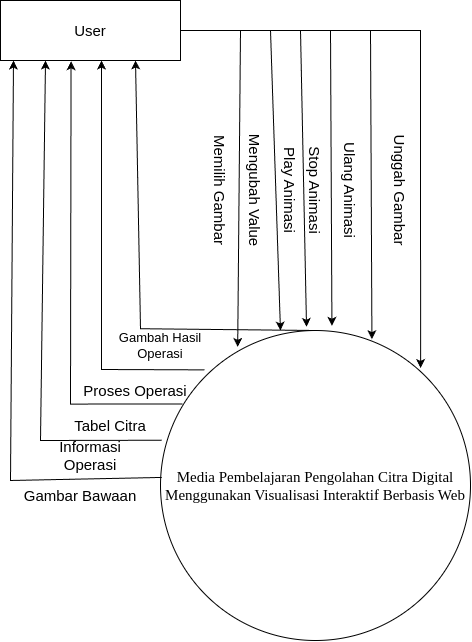
\includegraphics[width=0.6\textwidth, center]{images/diagram-konteks.png}
              \caption{\textit{Context Diagram} Media Pembelajaran pengolahan Citra Menggunakan Visualisasi Interaktif Berbasis Web}
          \end{figure*}

\textit{Context diagram} sangat berguna pada tahap awal perancangan sistem karena membantu para pemangku kepentingan memahami batasan dan lingkup sistem. Diagram ini juga memudahkan identifikasi entitas eksternal yang berinteraksi dengan sistem, seperti pengguna, perangkat lunak lain, atau sistem fisik. Dengan demikian, context diagram membantu menentukan kebutuhan fungsional dan non-fungsional sistem, serta menyekjdiakan dasar untuk perancangan lebih detail. Adapun Context diagram pada aplikasi media pembelajaran pengolahan citra digital berbasis web bisa dilihat pada gambar 3.1.


\item\textit{Hierarchy Chart}

\textit{Hierarchy chart} adalah sebuah alat visual yang digunakan untuk menggambarkan struktur hirarkis suatu sistem atau proses, menampilkan hubungan antara komponen atau modul dalam bentuk hierarki. Diagram ini sering digunakan dalam pengembangan perangkat lunak, perencanaan organisasi, dan manajemen proyek untuk memberikan pemahaman yang jelas mengenai bagaimana berbagai elemen berinteraksi dan berhubungan satu sama lain. \textit{Hierarchy chart} yang akan dibangun bisa dilihat pada gambar 3.2.

          \begin{figure*}[ht]
    	      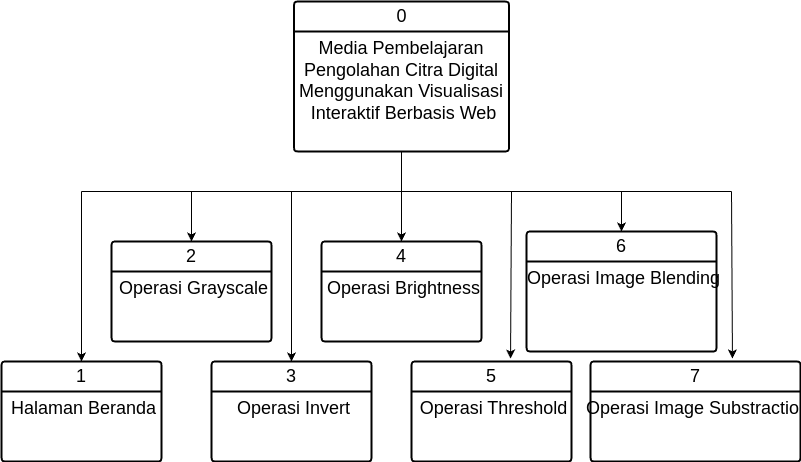
\includegraphics[width=15cm, center]{images/Hierarchy-Chart.png}
              \caption{\textit{Hierarchy Chart} Media Pembelajaran pengolahan Citra Menggunakan Visualisasi Interaktif Berbasis Web}
          \end{figure*}

\item\textit{Activity Diagram}

\textit{Activity diagram} adalah salah satu jenis diagram dalam Unified Modeling Language (UML) yang sangat berguna dalam memodelkan alur kerja atau proses bisnis yang terjadi di dalam sebuah sistem. Diagram ini memberikan representasi visual yang jelas dari berbagai aktivitas serta urutan tindakan yang berlangsung dalam sebuah proses, memperlihatkan bagaimana satu aktivitas mengarah dan bertransisi ke aktivitas lainnya. Hal ini, seperti yang dapat dilihat pada gambar 3.3, membantu dalam memahami serta menganalisis alur kerja secara lebih mendalam dan terstruktur.

       
          \begin{figure*}[ht]
    	      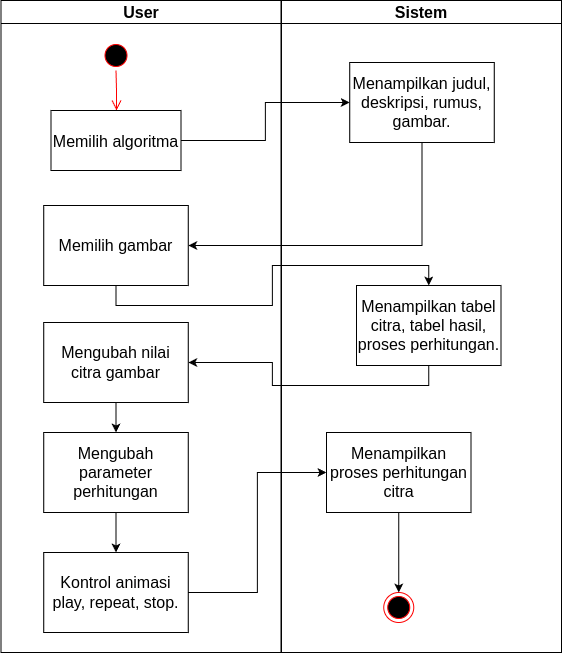
\includegraphics[width=8cm, center]{images/Activity-Diagram.png}
              \caption{\textit{Activity Diagram} Media Pembelajaran pengolahan Citra Menggunakan Visualisasi Interaktif Berbasis Web}
          \end{figure*}

      \item Program \textit{Flowchart}

Berikut adalah flowchart yang menunjukkan sistem media pembelajaran pengolahan citra digital berbasis web yang memperlihatkan alur atau langkah-langkah yang terjadi dalam sistem tersebut. Flowchart tersebut merupakan gambaran visual tentang bagaimana sistem media pembelaran tersebut beroperasi.

\begin{enumerate}[leftmargin=1cm, itemindent=0.6cm,labelwidth=15pt, labelsep=5pt, listparindent=1cm,align=left]

    \item Program Flowchart Operasi Grayscale

        Flowchart Operasi Grayscale adalah sebuah gambaran langkah demi langkah saat pengguna melakukan memulai proses mengubah tabel citra warna menjadi citra grayscale. Pada menu grayscale pengguna diminta memilih salah satu dari gambar kemudian pengguna bisa mengubah nilai dari citra warna tersebut. Jika pengguna tidak mengubah nilai dari citra warna pengguna bisa menekan tombol \textit{start, pause, stop} dan \textit{repeat}.

          \begin{figure*}[ht]
    	      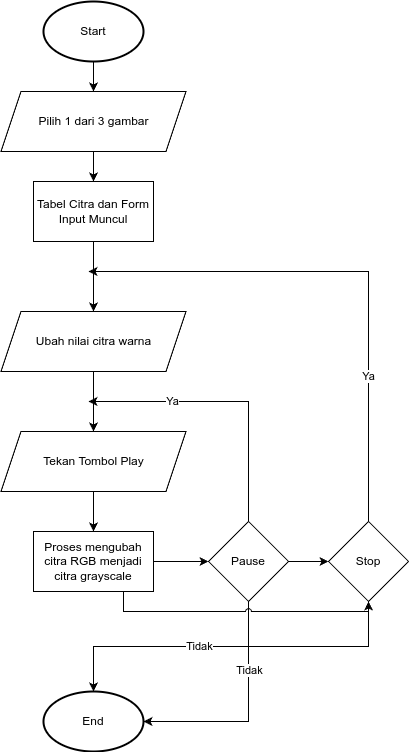
\includegraphics[width=0.5\textwidth, center]{images/flowchart-grayscale.png}
              \caption{\textit{Flowchart grayscale}}
          \end{figure*}

    \item Program Flowchart Operasi \textit{Invert}

        Flowchart Operasi \textit{Invert} atau negatif adalah sebuah gambaran langkah demi langkah saat pengguna melakukan memulai proses mengubah tabel citra grayscale menjadi citra negatif. Pada menu \textit{invert} pengguna diminta memilih salah satu dari gambar kemudian pengguna bisa mengubah nilai dari citra warna tersebut. Jika pengguna tidak mengubah nilai dari citra warna pengguna bisa menekan tombol \textit{start, pause, stop} dan \textit{repeat}.


      \begin{figure*}[ht]
          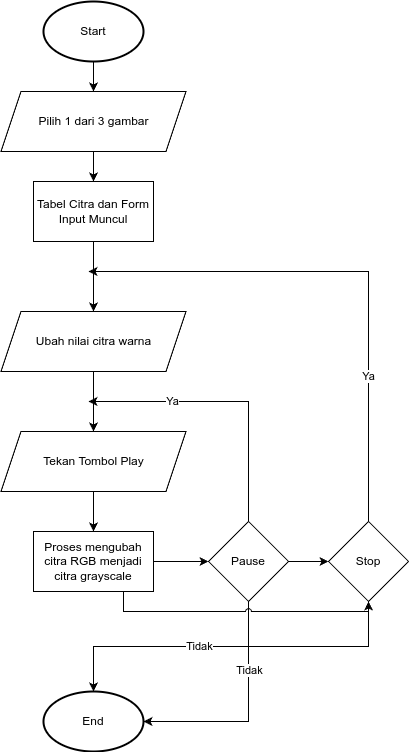
\includegraphics[width=0.5\textwidth, center]{images/flowchart-grayscale.png}
          \caption{\textit{Flowchart Invert}}
      \end{figure*}

    \item Program Flowchart Operasi \textit{Brightness}

    Flowchart Operasi \textit{Brightness} adalah sebuah gambaran langkah demi langkah saat pengguna melakukan memulai proses mengubah tabel citra grayscale menjadi citra dengan nilai baru yaitu peningkatan kecerahan. Pada menu \textit{brightness} pengguna diminta memilih salah satu dari gambar kemudian pengguna bisa mengubah nilai dari citra grayscale tersebut. Jika pengguna tidak mengubah nilai dari citra warna pengguna bisa menekan tombol \textit{start, pause, stop} dan \textit{repeat}. Pengguna juga bisa mengatur berapa besar konstanta yang akan ditingkatkan menggunakan \textit{slider ranger input}.

    \pagebreak

      \begin{figure*}[ht]
          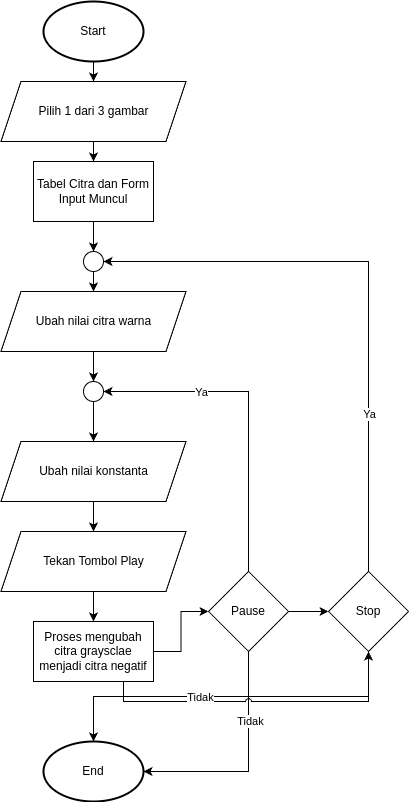
\includegraphics[width=0.5\textwidth, center]{images/flowchart-brightness.png}
          \caption{\textit{Flowchart Brightness}}
      \end{figure*}

    \item Program Flowchart Operasi \textit{Threshold}

    Flowchart operasi \textit{threshold} adalah sebuah gambaran langkah demi langkah saat pengguna melakukan memulai proses mengubah tabel citra grayscale menjadi citra dengan antara 0 atau 255. Pada menu \textit{threshold} pengguna diminta memilih salah satu dari gambar kemudian pengguna bisa mengubah nilai dari citra grayscale tersebut. Jika pengguna tidak mengubah nilai dari citra warna pengguna bisa menekan tombol \textit{start, pause, stop} dan \textit{repeat}. Pengguna juga bisa mengatur berapa besar nilai \(T\) yang akan ditingkatkan menggunakan \textit{input number}.

    \pagebreak

      \begin{figure*}[ht]
          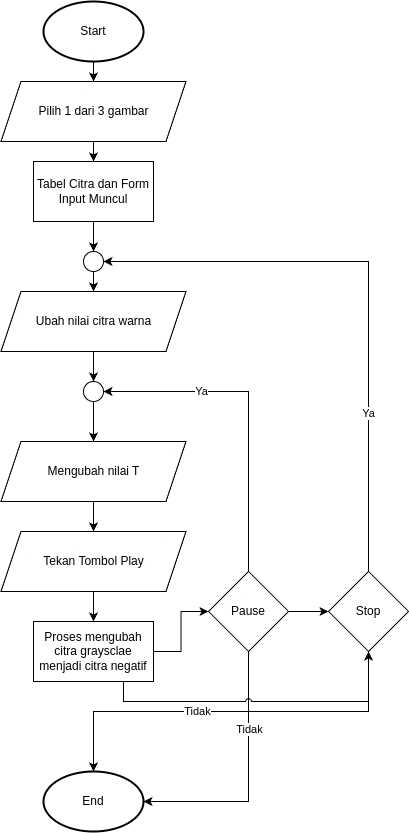
\includegraphics[width=0.5\textwidth, center]{images/flowchart-threshold.png}
          \caption{\textit{Flowchart Threshold}}
      \end{figure*}

    \item Program Flowchart Operasi \textit{Image Blending}

        Flowchart Operasi \textit{Image Blending} adalah sebuah gambaran langkah demi langkah saat pengguna melakukan memulai proses penjumlahan antara 2 citra grayscale. Pada menu \textit{image blending} pengguna diminta memilih 2 gambar kemudian pengguna bisa mengubah nilai dari citra grayscale tersebut. Jika pengguna tidak mengubah nilai dari citra warna pengguna bisa menekan tombol \textit{start, pause, stop} dan \textit{repeat}. Pengguna juga bisa mengatur berapa besar nilai \(\alpha\) antara 0.1 sampai dengan 0.9 menggunakan \textit{input number}.

    \pagebreak

      \begin{figure*}[ht]
          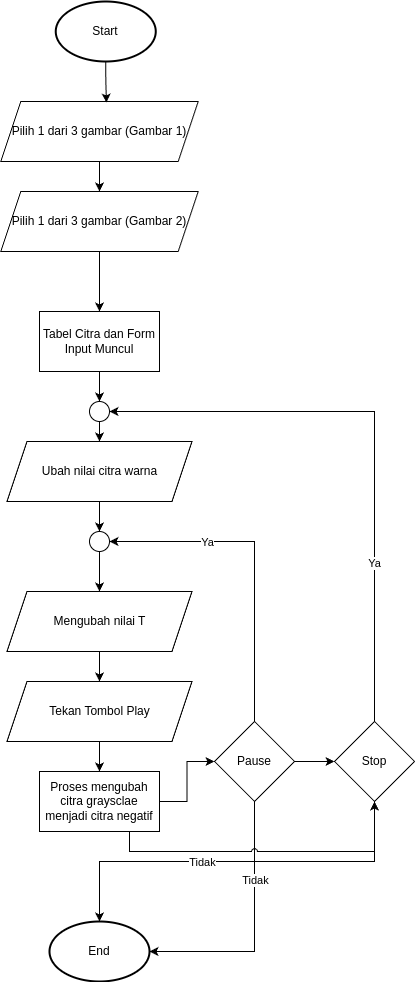
\includegraphics[width=0.5\textwidth, center]{images/flowchart-blending.png}
          \caption{\textit{Flowchart Image Blending}}
      \end{figure*}

    \item Program Flowchart Operasi \textit{Image Substraction}

    Flowchart Operasi \textit{Image Substraction} atau pengurangan citra adalah sebuah gambaran langkah demi langkah saat pengguna melakukan memulai proses pengurangan antara 2 citra grayscale. Pada menu \textit{image blending} pengguna diminta memilih 2 gambar kemudian pengguna bisa mengubah nilai dari citra grayscale tersebut. Jika pengguna tidak mengubah nilai dari citra warna pengguna bisa menekan tombol \textit{start, pause, stop} dan \textit{repeat}.

      \begin{figure*}[ht]
          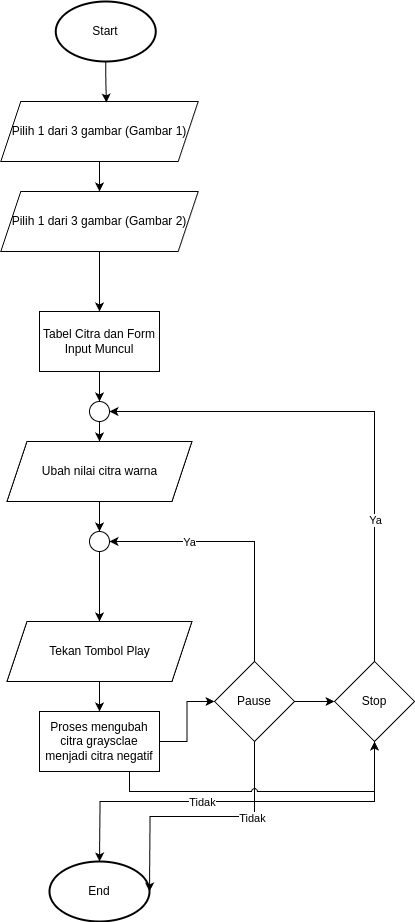
\includegraphics[width=0.5\textwidth, center]{images/flowchart-substraction.png}
          \caption{\textit{Flowchart Image Substraction}}
      \end{figure*}
\end{enumerate}

\item Desain Input

Desain input mengacu pada pengembangan antarmuka sistem yang melibatkan form input untuk pemrosesan operasi dan informasi yang inputkan akan mempengaruhi pada proses operasi itu sendiri.


\begin{enumerate}[leftmargin=1cm, itemindent=0.6cm,labelwidth=15pt, labelsep=5pt, listparindent=1cm,align=left]

    \item Desain input operasi \textit{grayscale}

Halaman ini adalah visualisasi pengolahan citra digital yang bertujuan mengubah gambar berwarna RGB menjadi grayscale. Terdapat beberapa elemen utama di halaman ini, mulai dari judul "Operasi RGB ke Grayscale" hingga deskripsi singkat tentang konversi warna.

Pengguna dapat memilih salah satu dari tiga gambar untuk diproses. Setelah memilih gambar, tabel RGB muncul dengan nilai awal, dan pengguna dapat mengubah nilai RGB melalui input text area.

          \begin{figure*}[ht]
    	      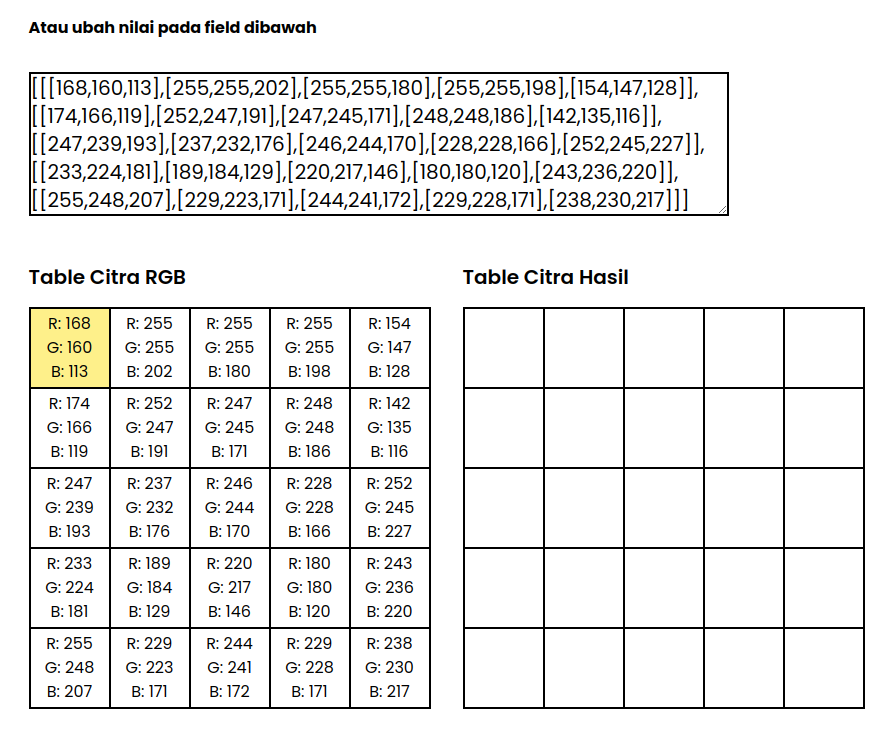
\includegraphics[width=0.6\textwidth, center]{images/input-grayscale.png}
              \caption{Desain Input Halaman \textit{Grayscale}}
          \end{figure*}

    \item Desain input operasi \textit{invert}

          \begin{figure*}[ht]
    	      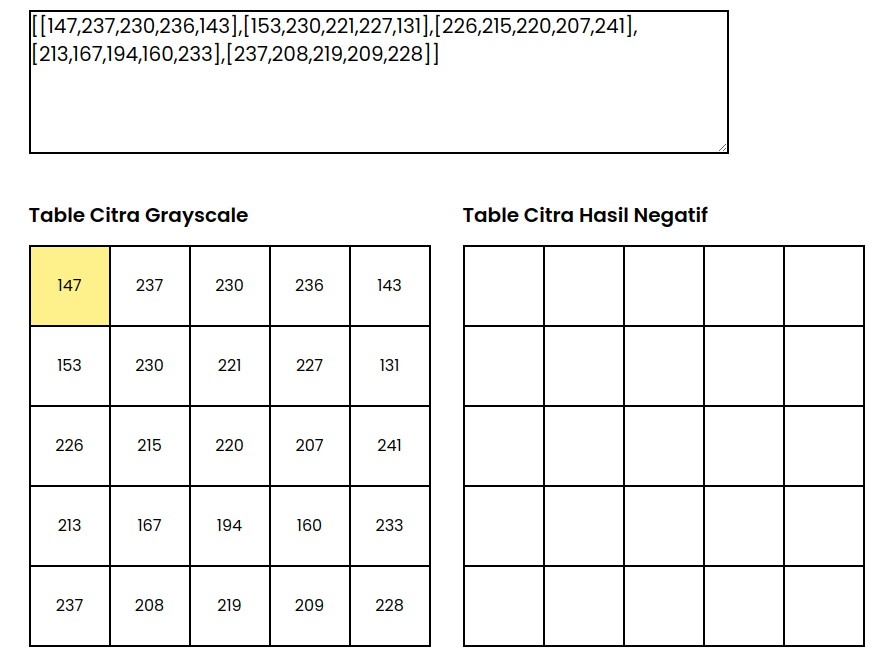
\includegraphics[width=0.6\textwidth, center]{images/input-invert.png}
              \caption{Desain Input Halaman \textit{Invert}}
          \end{figure*}

        Halaman ini adalah visualisasi pengolahan citra digital yang bertujuan mengubah gambar grayscale menjadi negatif. Terdapat beberapa elemen utama di halaman ini, mulai dari judul "Operasi Negatif", deskripsi singkat tentang konversi negatif, contoh kasus, tabel citra \textit{grayscale} serta tabel citra hasil.

Pengguna dapat memilih salah satu dari tiga gambar \textit{grayscale} untuk diproses. Setelah memilih gambar, tabel \textit{grayscale} muncul dengan nilai awal, dan pengguna dapat mengubah nilai \textit{grayscale} melalui input text area.

    \item Desain input operasi \textit{Brightness}

Untuk halaman ini yang bertujuan untuk mengubah kecerahan dari sebuah gambar. Terdapat beberapa element mulai dari judul, deskripsi singkat, rumus, tabel citra awal table citra hasil.

Pengguna dapat memilih salah satu dari tiga gambar \textit{grayscale} untuk diproses. Setelah memilih gambar, tabel \textit{grayscale} muncul dengan nilai awal, dan pengguna dapat mengubah nilai \textit{grayscale} melalui input text area. Pengguna juga dapat mengubah nilai konstanta menggunakan \textit{range slider}.

          \begin{figure*}[ht]
    	      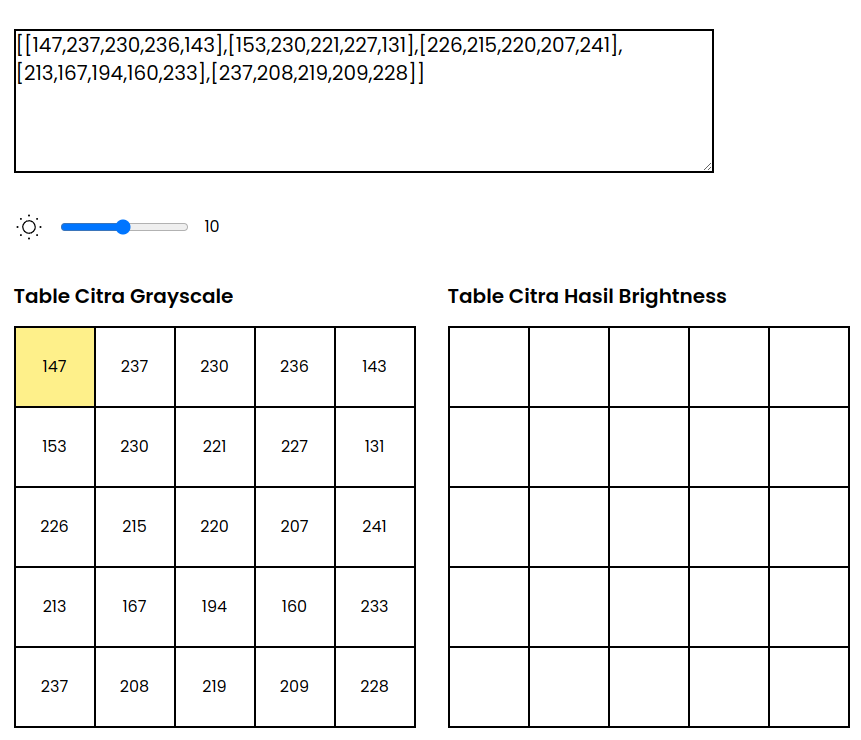
\includegraphics[width=0.6\textwidth, center]{images/input-brightness.png}
              \caption{Desain Input Halaman \textit{Brightness}}
          \end{figure*}

    \item Desain input operasi \textit{Threshold}

Pada halaman ini yang bertujuan untuk malukan proses ambang batas dari sebuah gambar. Terdapat beberapa element mulai dari judul, deskripsi singkat, rumus, tabel citra awal table citra hasil.

Pengguna dapat memilih salah satu dari tiga gambar \textit{grayscale} untuk diproses. Setelah memilih gambar, tabel \textit{grayscale} muncul dengan nilai awal, dan pengguna dapat mengubah nilai \textit{grayscale} melalui input text area. Pengguna juga dapat mengubah nilai \(T\) menggunakan \textit{input number}.

          \begin{figure*}[ht]
    	      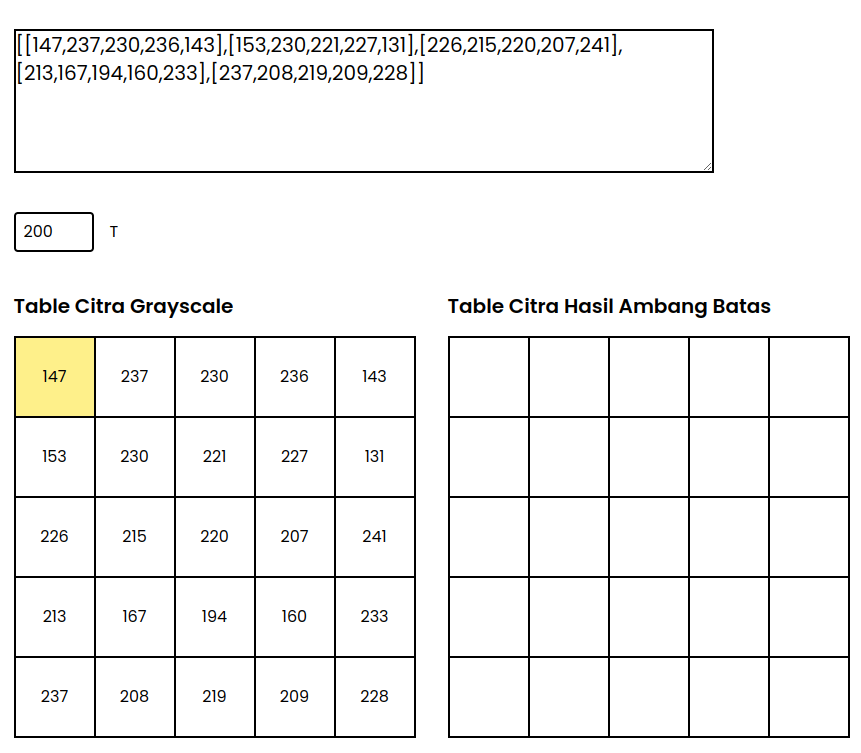
\includegraphics[width=0.8\textwidth, center]{images/input-threshold.png}
              \caption{Desain Input Halaman \textit{Threshold}}
          \end{figure*}

    \item Desain input operasi \textit{Image Blending}


          Halaman ini adalah visualisasi pengolahan citra digital yang bertujuan menggabungkan 2 buah citra. Terdapat beberapa elemen utama di halaman ini, mulai dari judul "Operasi Penjumlahan Citra", deskripsi singkat tentang \textit{image blending}, contoh kasus, 2 tabel citra \textit{grayscale} serta tabel citra hasil.

          Pengguna dapat memilih dua gambar \textit{grayscale} untuk diproses. Setelah memilih gambar, tabel \textit{grayscale} muncul dengan nilai awal, dan pengguna dapat mengubah nilai \textit{grayscale} melalui dua \textit{input text area}. Pengguna juga dapat menginput nilai \textit{threshold} dari angka 1 - 255.


          \begin{figure*}[ht]
    	      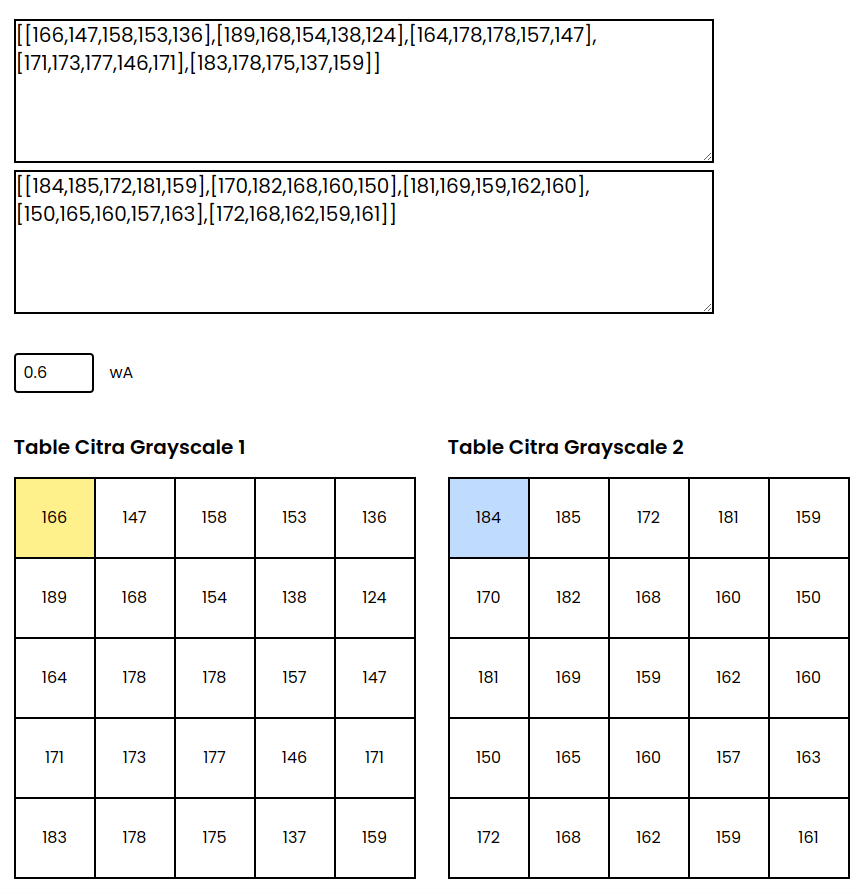
\includegraphics[width=0.6\textwidth, center]{images/input-blending.png}
              \caption{Desain Input Halaman \textit{Image Blending}}
          \end{figure*}

    \item Desain input operasi \textit{Image Substraction}

          Halaman ini adalah visualisasi pengolahan citra digital yang bertujuan mengurangi dua buah citra. Terdapat beberapa elemen utama di halaman ini, mulai dari judul "Operasi Pengurangan Citra", deskripsi singkat tentang \textit{image substraction}, contoh kasus, dua tabel citra \textit{grayscale} serta tabel citra hasil.

          Pengguna dapat memilih dua gambar \textit{grayscale} untuk diproses. Setelah memilih gambar, tabel \textit{grayscale} muncul dengan nilai awal, dan pengguna dapat mengubah nilai \textit{grayscale} melalui dua \textit{input text area}.

    \pagebreak

          \begin{figure*}[ht]
    	      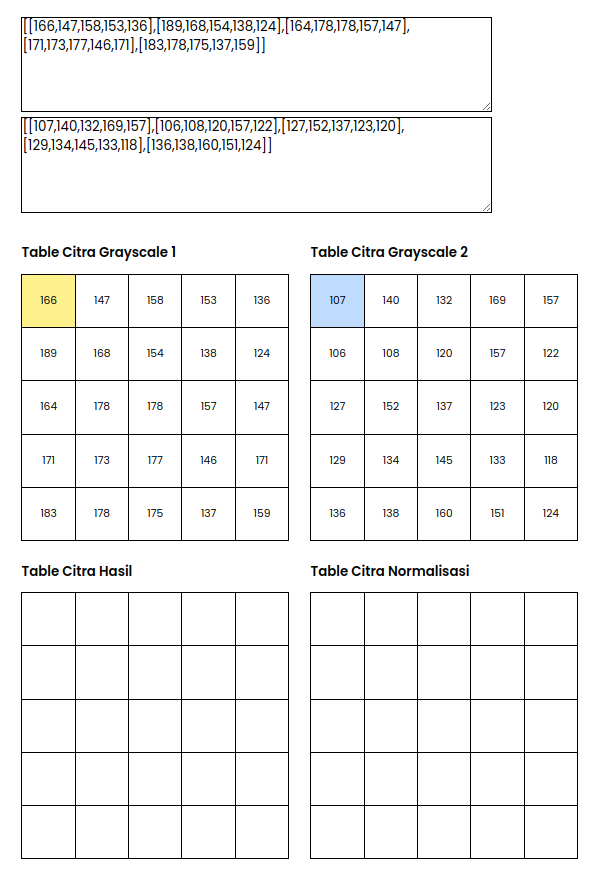
\includegraphics[width=0.6\textwidth, center]{images/input-substraction.png}
              \caption{Desain Input Halaman \textit{Image Substraction}}
          \end{figure*}
\end{enumerate}
\end{enumerate}

    \item Implementasi

    Tahap implementasi melibatkan pembuatan kode program berdasarkan perancangan yang telah disusun sebelumnya. Pada tahap ini, dilakukan pengembangan aplikasi berbasis web yang mendukung pengolahan citra digital dan visualisasi interaktif. Web yang dibuat menggunakan HTML, CSS, dan JavaScript, dengan React dan Tailwind CSS sebagai library tambahannya. Algoritma pengolahan citra yang dipilih akan diimplementasikan dalam kode program yang sesuai.

    \item Pengujian

    Setelah tahap implementasi, tahap pengujian dilakukan untuk memastikan bahwa aplikasi berfungsi dengan baik dan memenuhi kebutuhan pengguna. Pengujian dilakukan dengan menggunakan berbagai contoh kasus dan skenario untuk memverifikasi kinerja dan keakuratan media pembelajaran. Jika terdapat kesalahan atau kekurangan, perbaikan akan dilakukan pada tahap ini.

\item Pemeliharaan

    Setelah aplikasi diimplementasikan dan diuji, langkah selanjutnya adalah pemeliharaan. Tahap pemeliharaan melibatkan pemantauan kinerja aplikasi secara berkala dan memperbaiki masalah yang muncul setelah aplikasi berada dalam lingkungan produksi. Pemeliharaan juga mencakup penambahan fitur baru atau perubahan fungsionalitas sesuai dengan kebutuhan yang berkembang dari pengguna.

\end{enumerate}

Metode waterfall memberikan pendekatan yang terstruktur dan terurut dalam pengembangan aplikasi. Setiap tahap harus diselesaikan dengan baik sebelum melanjutkan ke tahap berikutnya. Pendekatan ini memastikan bahwa setiap fase pengembangan dapat diselesaikan dengan baik sebelum melanjutkan ke fase berikutnya, sehingga mengurangi risiko perubahan yang tidak terduga.

\section{Alat dan Bahan Penelitian}
\subsection{Spesifikasi Perangkat Keras(\textit{Hardware})}
    Perangkat keras (hardware) yang digunakan dalam pembangunan aplikasi media pebelajaran yang dibuat adalah sebagai berikut:
\begin{enumerate}
    \item \textit{Procesor AMD Ryzen 7 47000U with Raden Graphics 2.00 GHz}
    \item SSD 512 GB
    \item RAM 8 GB
\end{enumerate}

\subsection{Spesifikasi Perangkat Lunak(\textit{Software})}
    Perangkat Lunak (\textit{software}) yang digunakan dalam pembangunan aplikasi lowongan kerja yang dibangun adalah sebagai berikut:

\begin{enumerate}
    \item Sistem Operasi : Arch Linux
    \item Bahasa Pemrograman : Javascript
    \item Framework : Bootstrap
    \item Aplikasi desain logika program : draw.io
    \item Code Editor : Visual Studio Code
\end{enumerate}

    %-----------------------------------------------------------
    % End Daftar masukan untuk Bab
    %===========================================================

    %===========================================================
    % Daftar Pustaka
    %-----------------------------------------------------------
    \addcontentsline{toc}{chapter}{DAFTAR PUSTAKA}
    \printbibliography[title={DAFTAR PUSTAKA}]
    %-----------------------------------------------------------
    % End Daftar Pustaka
    %===========================================================

\end{document}
